\documentclass{article}

% NeurIPS style
    \usepackage[final]{style}

\usepackage{amsmath}
\usepackage{hyperref}
\usepackage{url}
\usepackage{amssymb}
\usepackage{booktabs}
\usepackage{graphicx}
\usepackage{float}
\usepackage{caption}

\title{A Reproducibility Study of SGD, SVRG, and SAGA on Regularized Logistic Regression}
\author{
  William Zhang \\
  Carnegie Mellon University \\
  \texttt{wz4@andrew.cmu.edu}
  \And
  Jihyun Kim \\
  Carnegie Mellon University \\
  \texttt{jihyunki@cmu.edu}
}

\begin{document}

\maketitle

\begin{abstract}
This project studies three stochastic optimization methods on the same convex
finite-sum problem: L2-regularized binary logistic regression on the
\texttt{sklearn} breast cancer dataset. The methods are stochastic gradient
descent (SGD), stochastic variance-reduced gradient (SVRG), and SAGA. The main
goal is not to claim a new algorithm, but to reproduce and compare the practical
behavior of these methods under one controlled setup. We evaluate convergence,
wall-clock runtime, gradient-evaluation cost, validation loss, stability across
random seeds, and memory usage. We also add a simple linear-convergence check by
plotting $F(\theta)-F^*$ on a log scale. The final results show that SVRG
reached the lowest training objective in the locked run, SAGA was competitive
with a tuned learning rate, and SGD was the cheapest method in memory and
gradient work.
\end{abstract}

\section{Introduction}

Stochastic gradient methods are a standard tool for machine learning
optimization. They are attractive because each update can be much cheaper than
computing a full gradient over the whole dataset. The downside is that a single
sample gradient is noisy. This noise can make the objective decrease unevenly,
especially when the method gets close to a good solution.

Variance-reduced methods try to keep the low per-iteration cost of stochastic
methods while making the update direction more reliable. In this project, we
compare plain SGD with two variance-reduced methods, SVRG and SAGA. The study is
set up as a paper reading and reproducibility project rather than a new method
proposal. The goal is to implement the algorithms, run them on a clean convex
problem, and understand the tradeoffs that appear in practice.

The problem we use is L2-regularized logistic regression on the breast cancer
dataset from \texttt{sklearn}. This is a useful test case because the objective
is convex, the dataset is small enough to inspect carefully, and the finite-sum
structure matches the setting where SVRG and SAGA are usually discussed. We
focus on four practical questions:
\begin{itemize}
    \item Which method reduces the objective fastest at the beginning?
    \item Which method reaches the best final objective value?
    \item How much do the methods differ in runtime and gradient evaluations?
    \item Do the variance-reduced methods show the expected linear-convergence
    pattern on a log-scale excess-loss plot?
    \item How do validation loss, memory cost, and stability change when using
    variance reduction?
\end{itemize}

\section{Background and Motivation}

For empirical risk minimization problems, the objective often has the form
\[
F(\theta) = \frac{1}{n}\sum_{i=1}^{n} f_i(\theta) + r(\theta),
\]
where $f_i$ is the loss for one training example and $r$ is a regularization
term. Full gradient descent uses all $n$ examples for every update, which gives
a stable direction but can be expensive for large datasets. SGD instead samples
one example, or a mini-batch, and uses that gradient as an estimate of the full
gradient.

The main motivation for SVRG and SAGA is that the stochastic gradient in SGD can
have high variance. Even when the current point is near the optimum, a single
sample gradient may point in a noticeably different direction from the full
gradient. Because of this, SGD often needs a decreasing learning rate or it
keeps fluctuating near the solution.

Variance-reduced methods use extra information to reduce this noise. SVRG uses
periodic full-gradient calculations at a snapshot point. SAGA stores past
per-sample gradients and uses their average as a correction. Both methods spend
extra resources to get a better update direction. In strongly convex finite-sum
settings, this is also the high-level reason these methods can show linear
convergence, meaning the optimization error shrinks by a roughly constant factor
per pass after the method is in its stable regime.

I do not prove any new theoretical results in this project. The relevant theory
from the literature says, roughly, that variance-reduced methods can improve the
convergence behavior for finite-sum convex problems because their gradient
estimates become more accurate as the iterates approach a solution. I use that
theory as motivation and check it empirically by plotting $F(\theta)-F^*$,
where $F^*$ is estimated with a high-precision L-BFGS-B solve.

\section{Problem Formulation}

The dataset is \texttt{sklearn.datasets.load\_breast\_cancer}. It has
569 samples and 30 features. The
features are standardized before optimization. The original binary labels are
converted to
\[
y_i \in \{-1,+1\}.
\]
After conversion, the class counts are 212 samples with label $-1$ and 357
samples with label $+1$.
For the validation-loss experiment, I use a stratified 80/20 split. This gives
455 training samples and 114 validation samples. The scaler is fit on the
training set and then applied to the validation set.

The model is binary logistic regression with parameters $w \in \mathbb{R}^d$
and bias $b \in \mathbb{R}$. The objective is
\[
F(w,b)
= \frac{1}{n}\sum_{i=1}^{n}
\log\left(1+\exp\left(-y_i(w^\top x_i+b)\right)\right)
+ \frac{\lambda}{2}\|w\|_2^2 .
\]
The regularization parameter is
\[
\lambda = 10^{-3}.
\]
The bias term is not regularized.

For implementation, I store the parameters as one vector
\[
\theta = (w,b) \in \mathbb{R}^{d+1}.
\]
The full gradient is used for objective checking and for SVRG snapshot steps.
The per-sample gradient is used by all three stochastic methods. I also checked
the gradient implementation numerically using finite differences:
\[
\text{maximum finite difference error} = 7.173 \times 10^{-11}.
\]
This check is important because a small gradient bug would make the algorithm
comparison meaningless.

\section{Methods}

\subsection{SGD}

SGD is the baseline method. At each step, it samples one index $i_t$ uniformly
from the training set and updates
\[
\theta_{t+1} = \theta_t - \eta \nabla f_{i_t}(\theta_t),
\]
where $\eta$ is the learning rate. In this project, I use a constant learning
rate for each run and tune it with a small grid search.

The main advantage of SGD is simplicity. It uses one sample gradient per update
and has very low memory cost. The main disadvantage is that the update direction
is noisy. In the results, I expect SGD to make fast early progress but to be
less smooth near the final objective value.

\subsection{SVRG}

SVRG uses a snapshot parameter $\tilde{\theta}$. At the start of each outer
loop, it computes the full gradient $\nabla F(\tilde{\theta})$. Then, inside
the inner loop, it samples an index $i_t$ and uses
\[
v_t =
\nabla f_{i_t}(\theta_t)
- \nabla f_{i_t}(\tilde{\theta})
+ \nabla F(\tilde{\theta}).
\]
The update is
\[
\theta_{t+1} = \theta_t - \eta v_t.
\]

The correction term makes the stochastic update closer to the full-gradient
direction while still using a sampled index in the inner loop. In the locked
train/validation experiment, the inner loop length is 455, which is one pass
over the training set. The tradeoff is that SVRG does not store a large table
of gradients, but it does pay for repeated full-gradient computations.

\subsection{SAGA}

SAGA keeps a table of stored gradients, one for each training example. At each
step, it samples an index, computes the current per-sample gradient for that
index, and combines it with the stored table average. A simple way to write the
update direction is
\[
v_t =
\nabla f_{i_t}(\theta_t)
- \alpha_{i_t}
+ \frac{1}{n}\sum_{j=1}^{n}\alpha_j,
\]
where $\alpha_j$ is the stored gradient for sample $j$. After the update, the
table entry for $i_t$ is replaced by the new gradient.

In my implementation, the table stores the unregularized per-sample logistic
loss gradients, and the L2 regularization gradient is added using the current
$w$. This keeps the stored table from depending on an old value of the
regularization term.

SAGA's main cost is memory. It stores an $n \times (d+1)$ gradient table, so the
storage grows with both the number of examples and the number of features. On
the breast cancer dataset this is small, but the scaling is important when
thinking about larger problems.

\section{Experimental Setup}

All methods use the same objective, preprocessing, initialization, and stopping
condition. The initial parameter vector is the zero vector. Each run uses 30
epochs. I record the training objective after each epoch, along with the
cumulative number of gradient evaluations and the wall-clock runtime. For the
train/validation run, I also record the validation objective at the same
checkpoints.

The learning-rate grids are:
\[
\text{SGD: } \{0.001, 0.003, 0.01, 0.03, 0.1\},
\]
\[
\text{SVRG: } \{0.005, 0.01, 0.03, 0.05, 0.1, 0.2\},
\]
\[
\text{SAGA: } \{0.005, 0.01, 0.03, 0.05, 0.1, 0.2\}.
\]
After the sweep, I choose one learning rate per method for the locked
comparison:
\[
\eta_{\text{SGD}} = 0.03, \quad
\eta_{\text{SVRG}} = 0.1, \quad
\eta_{\text{SAGA}} = 0.03.
\]

The main metrics are:
\begin{itemize}
    \item final objective value,
    \item objective value versus gradient evaluations,
    \item objective value versus runtime,
    \item excess objective $F(\theta)-F^*$ on a log scale,
    \item validation objective versus gradient evaluations,
    \item sensitivity to learning rate,
    \item stability across seeds,
    \item memory usage of the optimizer state.
\end{itemize}

The saved seed experiment uses seeds 0, 1, and 2. I use this experiment to
check whether one method is consistently better or whether the result is mainly
due to one lucky random run. The current seed CSV contains SGD and SVRG, so I
only report seed statistics for those two methods.

\section{Numerical Results}

\subsection{Learning-Rate Sweep}

Before comparing the methods directly, I first tune the learning rate for each
method. Table~\ref{tab:lr-sweep} reports the best learning rate from the sweep
for each method. The full sweep is shown visually in
Figure~\ref{fig:lr-sweep} and is also saved in
\texttt{outputs/lr\_sweep\_summary.csv}. This sweep was run on the full
standardized dataset and was used to choose the locked step sizes.

\begin{table}[H]
\centering
\caption{Best learning rates from the sweep with 30 epochs and seed 0.}
\label{tab:lr-sweep}
\begin{tabular}{lrrrr}
\toprule
Method & Learning rate & Final loss & Gradient evals & Runtime (s) \\
\midrule
SVRG & 0.100 & 0.0598532343 & 51210 & 0.3574 \\
SGD  & 0.030 & 0.0641138605 & 17070 & 0.2065 \\
SAGA & 0.030 & 0.0603328688 & 17639 & 0.2579 \\
\bottomrule
\end{tabular}
\end{table}

The sweep shows that all three methods need a reasonable learning rate. For
SGD, 0.03 gave the best final loss, while 0.1 was already too aggressive. For
SVRG, 0.1 gave the best final loss, but 0.2 made the result worse. For SAGA,
the best swept learning rate was 0.03. This matters because SAGA at 0.03
reached a final loss close to SVRG while using many fewer gradient evaluations.

\begin{figure}[H]
\centering
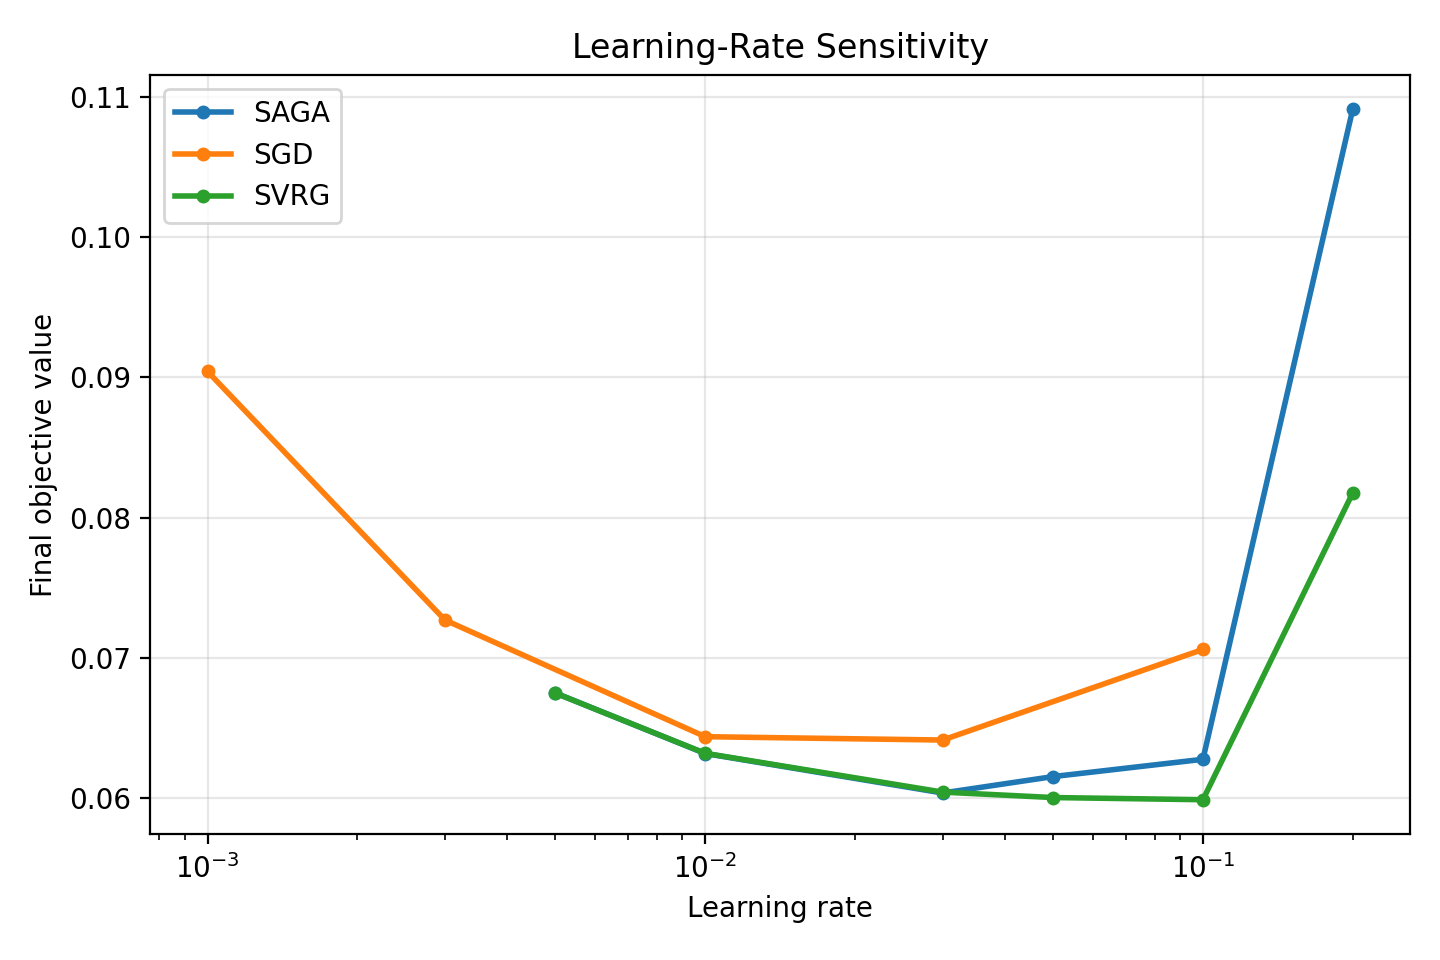
\includegraphics[width=0.58\textwidth]{outputs/lr_sweep_final_loss.png}
\caption{Learning-rate sensitivity for SGD, SVRG, and SAGA.}
\label{fig:lr-sweep}
\end{figure}

Figure~\ref{fig:lr-sweep} gives a visual check of the sweep. This figure is
useful because it shows whether each method has a wide stable range or only
works well for a narrow set of learning rates. In this experiment, the
variance-reduced methods improved a lot when moving from very small learning
rates to moderate ones, but both SVRG and SAGA became worse at 0.2. This was
the clearest sign that the step size still matters even when variance reduction
is used.

\subsection{Main Comparison}

After choosing the learning rates, I compare the three methods in one locked
run. Table~\ref{tab:main} includes the final objective, runtime, and
gradient-evaluation count for each method.

\begin{table}[H]
\centering
\caption{Main locked train-split comparison with seed 0.}
\label{tab:main}
\begin{tabular}{lrrrr}
\toprule
Method & Learning rate & Final loss & Gradient evals & Runtime (s) \\
\midrule
SGD  & 0.03 & 0.0586549325 & 13650 & 0.1335 \\
SVRG & 0.10 & 0.0557996994 & 40950 & 0.2987 \\
SAGA & 0.03 & 0.0566544845 & 14105 & 0.1576 \\
\bottomrule
\end{tabular}
\end{table}

This table is the main numerical summary of the project. It shows the basic
tradeoff between objective quality, runtime, and gradient-evaluation cost.
SVRG reached the lowest final training objective value, but it used about three
times as many gradient evaluations as SGD. SGD had the fastest runtime in this
locked run. SAGA used almost the same gradient-evaluation budget as SGD, after
its initial table setup, and ended between SGD and SVRG.

\begin{figure}[H]
\centering
\begin{minipage}{0.48\textwidth}
\centering
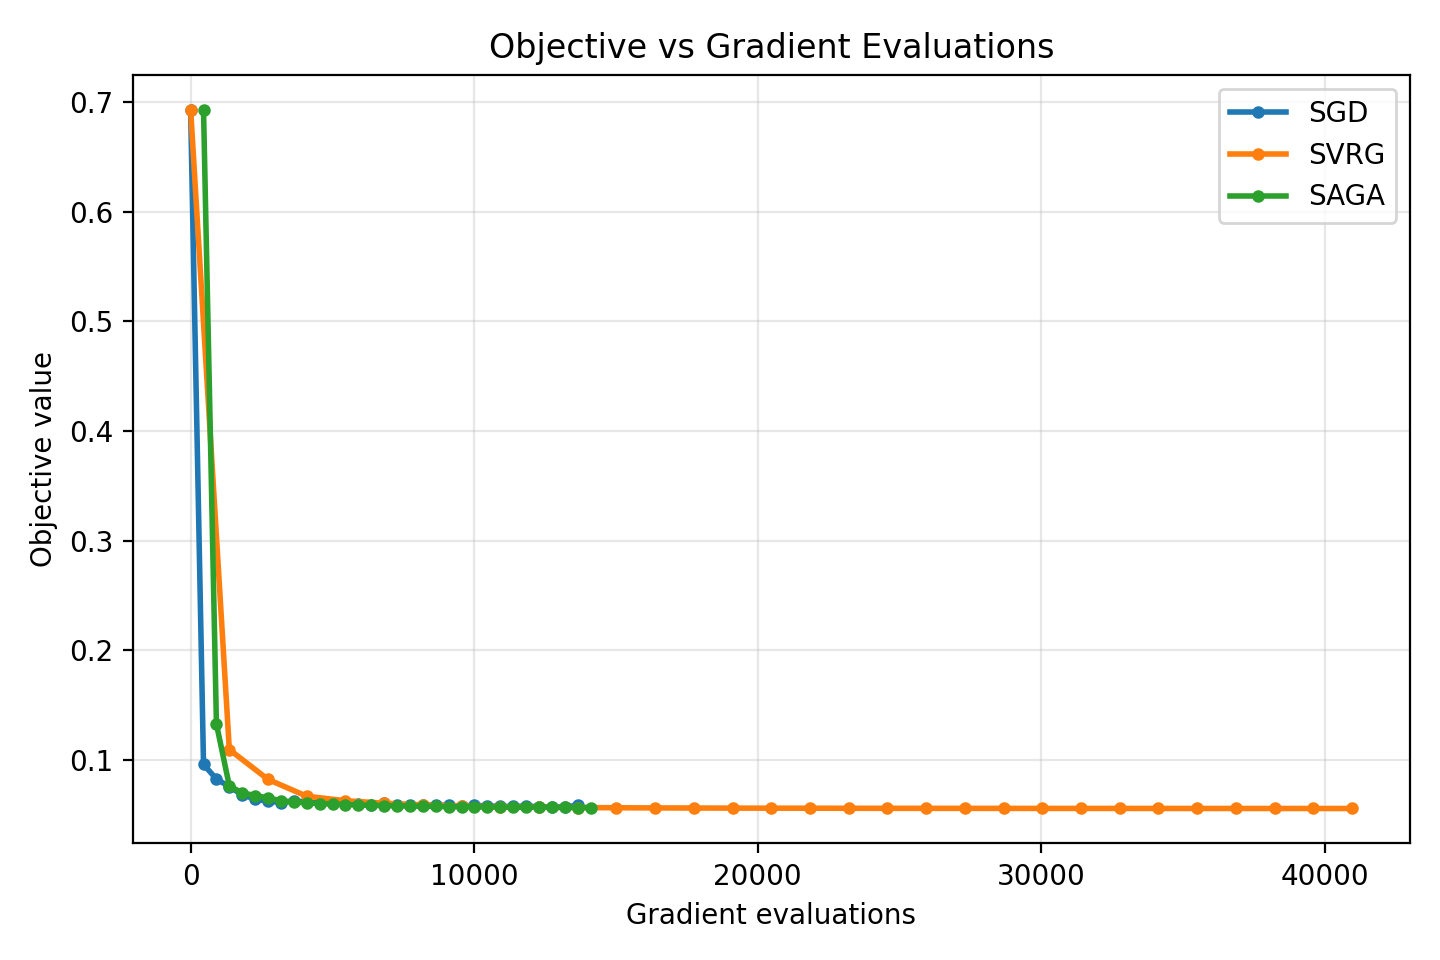
\includegraphics[width=\textwidth]{outputs/sgd_vs_svrg_loss_vs_grad_evals.png}
\small (a) Objective vs. gradient evaluations
\end{minipage}
\hfill
\begin{minipage}{0.48\textwidth}
\centering
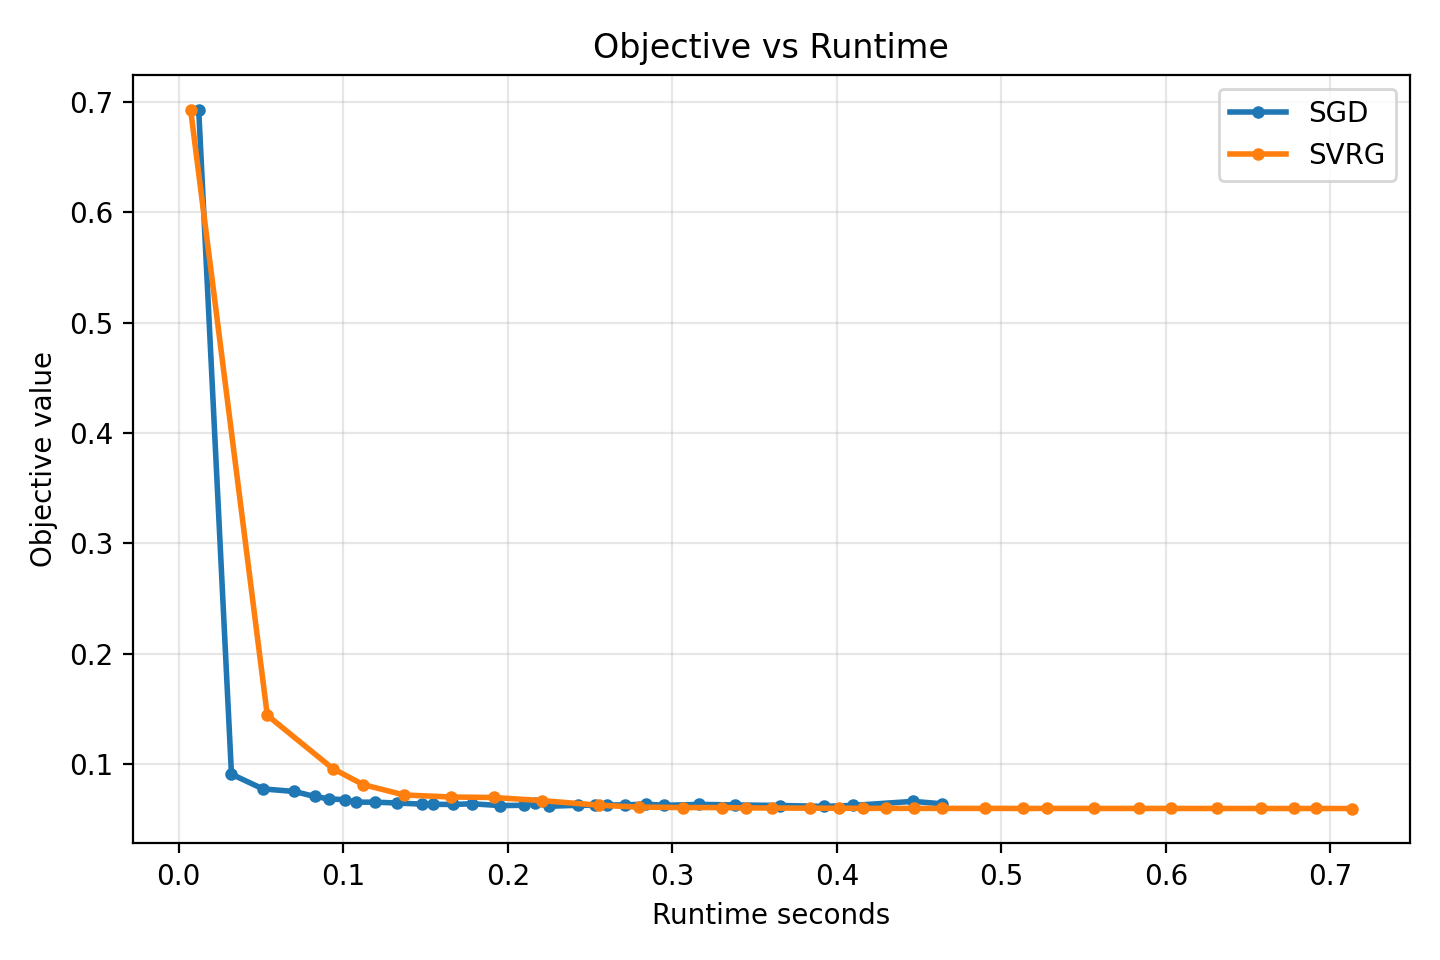
\includegraphics[width=\textwidth]{outputs/sgd_vs_svrg_loss_vs_runtime.png}
\small (b) Objective vs. runtime
\end{minipage}
\caption{Locked-run training objective curves.}
\label{fig:main-curves}
\end{figure}

Figure~\ref{fig:main-curves} compares the methods by gradient-evaluation cost
and by runtime. SGD gets a large drop very quickly, but then its curve is noisy
and it settles at a higher objective. SVRG decreases more smoothly and reaches
the best final value, but it spends many more gradient evaluations. SAGA has a
fast initial drop and ends between SGD and SVRG. In runtime, SGD is still the
fastest locked run, while SVRG takes longer because of the repeated full-gradient
computations.

\subsection{Linear Convergence and Validation Loss}

To address the linear-convergence feedback, I estimate the best training
objective value with L-BFGS-B and get
\[
F^* \approx 0.0557588295.
\]
Then I plot the excess objective $F(\theta)-F^*$ on a log scale. A method with
linear convergence should look roughly like a straight downward line on this
plot, while plain SGD with a constant step size should eventually flatten near
a noise floor.

\begin{figure}[H]
\centering
\begin{minipage}{0.48\textwidth}
\centering
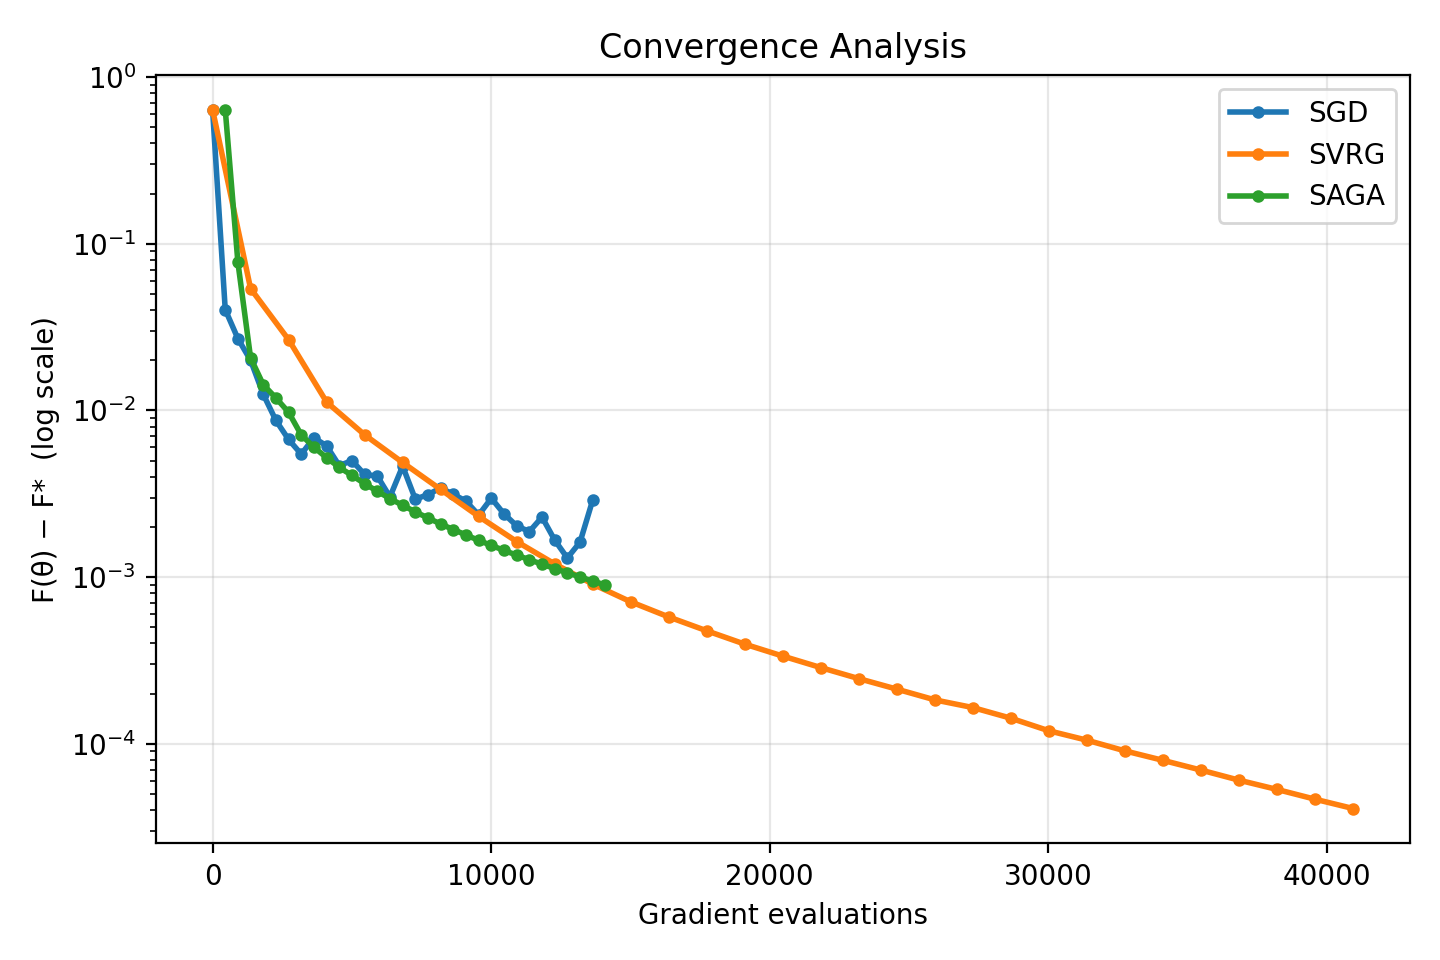
\includegraphics[width=\textwidth]{outputs/convergence_analysis.png}
\small (a) Excess training objective
\end{minipage}
\hfill
\begin{minipage}{0.48\textwidth}
\centering
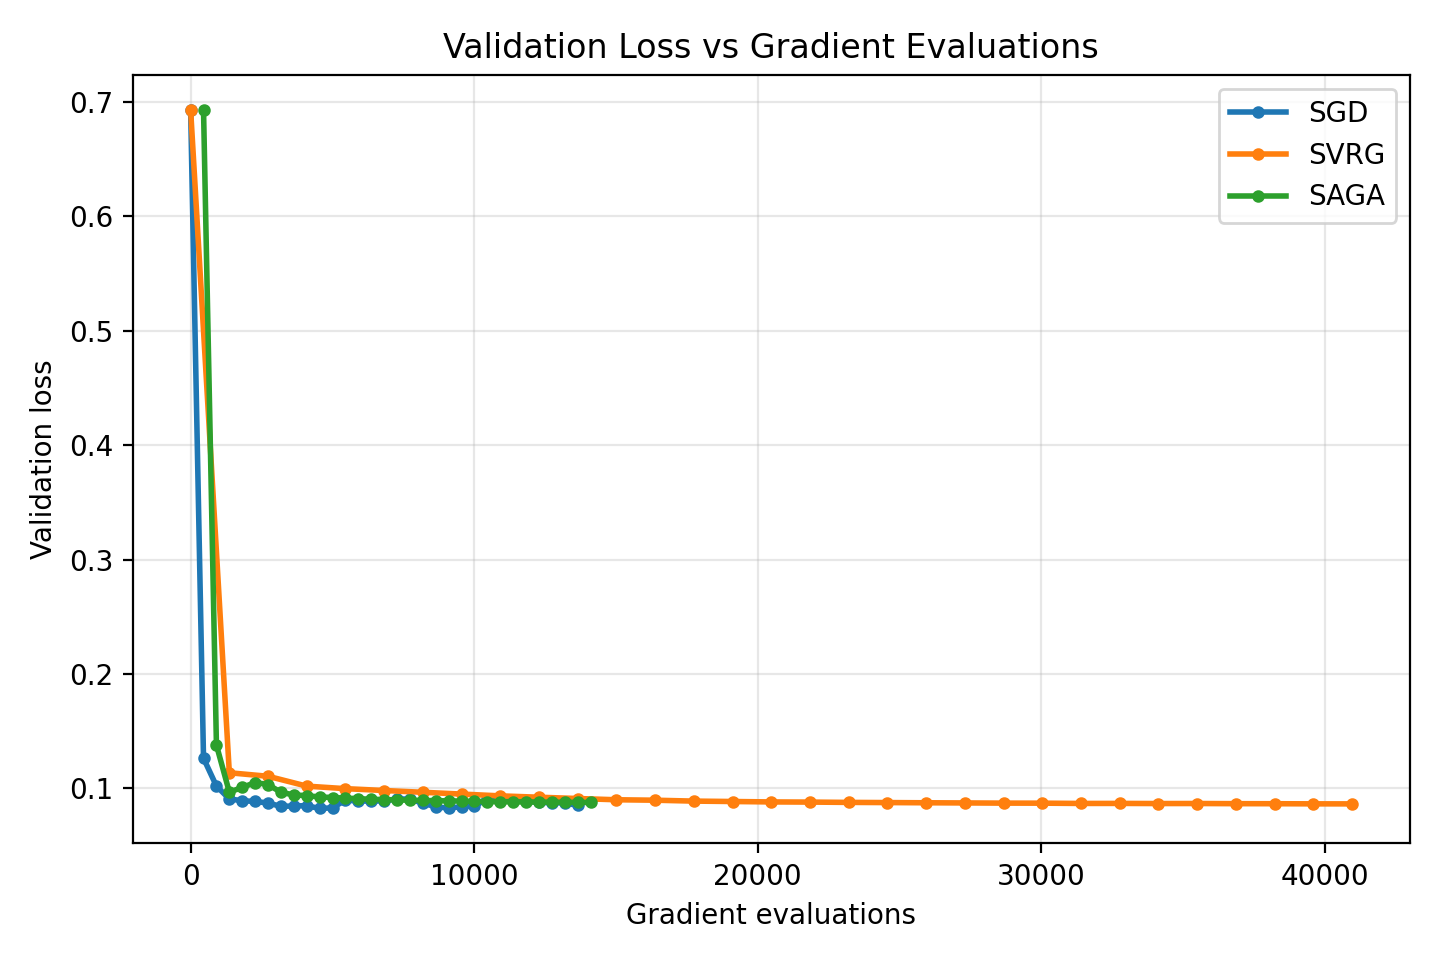
\includegraphics[width=\textwidth]{outputs/val_loss_vs_grad_evals.png}
\small (b) Validation objective
\end{minipage}
\caption{Linear-convergence and validation-loss checks.}
\label{fig:linear-validation}
\end{figure}

Figure~\ref{fig:linear-validation} matches the expected qualitative behavior on
the training objective. SVRG has the smallest final excess objective, about
$4.09 \times 10^{-5}$. SAGA also keeps decreasing and ends with excess objective
about $8.96 \times 10^{-4}$. SGD improves quickly at first, but its final excess
objective is larger, about $2.90 \times 10^{-3}$. On the validation split, the
final objectives are close: 0.0851 for SGD, 0.0865 for SVRG, and 0.0877 for
SAGA. I do not read this as a strong generalization win for any method.

\subsection{Stability Across Seeds}

Table~\ref{tab:seeds} reports the saved three-seed summary file. This seed
summary was run on the full dataset and currently contains SGD and SVRG results
for seeds 0, 1, and 2.

\begin{table}[H]
\centering
\caption{Seed stability summary from seeds 0, 1, and 2.}
\label{tab:seeds}
\begin{tabular}{lrrrr}
\toprule
Method & Mean final loss & Std. final loss & Mean runtime (s) & Mean grad evals \\
\midrule
SGD  & 0.0625934339 & 0.0013355237 & 0.3879 & 17070 \\
SVRG & 0.0598533388 & 0.0000094993 & 0.6513 & 51210 \\
\bottomrule
\end{tabular}
\end{table}

For the two reported methods, SVRG had a much smaller final-loss standard
deviation than SGD. I do not report a SAGA seed statistic because it is not in
the saved seed summary file.

\subsection{Memory and Compute Tradeoff}

The dataset itself is shared by all methods, so the memory comparison in
Table~\ref{tab:tradeoff} focuses on optimizer state.

\begin{table}[H]
\centering
\caption{Memory and compute tradeoff summary.}
\label{tab:tradeoff}
\small
\begin{tabular}{lp{0.18\textwidth}p{0.27\textwidth}p{0.33\textwidth}}
\toprule
Method & Extra memory & Extra compute pattern & Practical comment \\
\midrule
SGD  & about 0.5 KB & one sample gradient per step & lowest memory, noisy final behavior \\
SVRG & about 1.2 KB & periodic full gradients & best final loss, highest grad evals \\
SAGA & about 110.9 KB & stored gradient table & good tuned loss, largest memory \\
\bottomrule
\end{tabular}
\end{table}

For this dataset, SAGA's memory use is still small in absolute terms. The
important point is scaling: SAGA grows with $n(d+1)$, while SGD and SVRG use
only small $O(d)$ optimizer state.

\section{Discussion / Take-Home Messages}

Variance reduction helped, but the benefit was not free.
\begin{itemize}
    \item \textbf{Fastest early progress:} SGD and SAGA made the largest early
    drops; SGD was especially cheap in gradient evaluations.
    \item \textbf{Best final training objective:} SVRG had the best locked
    training loss, 0.0557996994. SAGA was second at 0.0566544845.
    \item \textbf{Validation loss:} the final validation objectives were close:
    0.0851 for SGD, 0.0865 for SVRG, and 0.0877 for SAGA.
    \item \textbf{Linear-convergence check:} SVRG and SAGA showed clearer
    continued decrease in $F(\theta)-F^*$ than constant-step-size SGD.
    \item \textbf{Most stable method:} For saved seed results, SVRG was most
    stable: $9.4993 \times 10^{-6}$ final-loss standard deviation versus
    $1.3355 \times 10^{-3}$ for SGD.
    \item \textbf{Lowest memory cost:} SGD used the least memory. SAGA used the
    most because of its gradient table.
    \item \textbf{Practical choice:} SGD is best for simplicity, SVRG for the
    lowest objective when full-gradient passes are affordable, and SAGA when the
    gradient table fits in memory and the step size is tuned.
\end{itemize}
The main limitation is that this is one small convex dataset, so the results
are a controlled tradeoff study rather than a universal benchmark.

\section{Conclusion}

SVRG gave the best final training objective value and the clearest
linear-convergence behavior, SGD was the cheapest and fastest locked baseline,
and SAGA became competitive when its learning rate was tuned carefully. The
validation losses were close across methods, so the main benefit of variance
reduction in this experiment is optimization behavior rather than a clear
validation-loss improvement. The practical lesson is that variance reduction can
help on this convex finite-sum problem, but it trades off against extra gradient
work for SVRG or extra memory for SAGA.

{
\small
\section*{References}

\noindent [1] A. Defazio, F. Bach, and S. Lacoste-Julien. SAGA: A Fast
Incremental Gradient Method With Support for Non-Strongly Convex Composite
Objectives. 2014.

\noindent [2] R. Johnson and T. Zhang. Accelerating Stochastic Gradient Descent
using Predictive Variance Reduction. 2013.

\noindent [3] H. Robbins and S. Monro. A Stochastic Approximation Method. 1951.

\noindent [4] L. Bottou, F. E. Curtis, and J. Nocedal. Optimization Methods for
Large-Scale Machine Learning. 2018.
}
\newpage

\end{document}
